%%%%%%%%%%%%%%%%%%%%%%%%%%%%%%%%%%%%%%%%%%%%%%%%%%%%%%%%%%%%%%%%%
% MUW Presentation
% LaTeX Template
% Version 1.0 (27/12/2016)
%
% License:
% CC BY-NC-SA 4.0 (http://creativecommons.org/licenses/by-nc-sa/3.0/)
%
% Created by:
% Nicolas Ballarini, CeMSIIS, Medical University of Vienna
% nicoballarini@gmail.com
% http://statistics.msi.meduniwien.ac.at/
%
% Customized for UAH by:
% David F. Barrero, Departamento de Automática, UAH
%%%%%%%%%%%%%%%%%%%%%%%%%%%%%%%%%%%%%%%%%%%%%%%%%%%%%%%%%%%%%%%%%

\documentclass[10pt,compress]{beamer} % Change 10pt to make fonts of a different size
\mode<presentation>

\usepackage[spanish]{babel}
\usepackage{fontspec}
\usepackage{tikz}
\usepackage{etoolbox}
\usepackage{xcolor}
\usepackage{xstring}
\usepackage{listings}

\usetheme{UAH}
\usecolortheme{UAH}
\setbeamertemplate{navigation symbols}{} 
\setbeamertemplate{caption}[numbered]

%%%%%%%%%%%%%%%%%%%%%%%%%%%%%%%%%%%%%%%%%%%%%%%%%%%%%%%%%%%%%%%%%
%% Presentation Info
\title[OOP concepts]{Object-Oriented Programming in Java}
\author{\asignatura\\\carrera}
\institute{}
\date{Departamento de Automática}
%%%%%%%%%%%%%%%%%%%%%%%%%%%%%%%%%%%%%%%%%%%%%%%%%%%%%%%%%%%%%%%%%


%%%%%%%%%%%%%%%%%%%%%%%%%%%%%%%%%%%%%%%%%%%%%%%%%%%%%%%%%%%%%%%%%
%% Descomentar para habilitar barra de navegación superior
\setNavigation
%%%%%%%%%%%%%%%%%%%%%%%%%%%%%%%%%%%%%%%%%%%%%%%%%%%%%%%%%%%%%%%%%

%%%%%%%%%%%%%%%%%%%%%%%%%%%%%%%%%%%%%%%%%%%%%%%%%%%%%%%%%%%%%%%%%
%% Configuración de logotipos en portada
%% Opacidad de los logotipos
\newcommand{\opacidad}{1}
%% Descomentar para habilitar logotipo en pié de página de portada
\renewcommand{\logoUno}{Images/isg.png}
%% Descomentar para habilitar logotipo en pié de página de portada
%\renewcommand{\logoDos}{Images/CCLogo.png}
%% Descomentar para habilitar logotipo en pié de página de portada
%\renewcommand{\logoTres}{Images/ALogo.png}
%% Descomentar para habilitar logotipo en pié de página de portada
%\renewcommand{\logoCuatro}{Images/ELogo.png}
%%%%%%%%%%%%%%%%%%%%%%%%%%%%%%%%%%%%%%%%%%%%%%%%%%%%%%%%%%%%%%%%%

%%%%%%%%%%%%%%%%%%%%%%%%%%%%%%%%%%%%%%%%%%%%%%%%%%%%%%%%%%%%%%%%%
%% FOOTLINE
%% Comment/Uncomment the following blocks to modify the footline
%% content in the body slides. 


%% Option A: Title and institute
\footlineA
%% Option B: Author and institute
%\footlineB
%% Option C: Title, Author and institute
%\footlineC
%%%%%%%%%%%%%%%%%%%%%%%%%%%%%%%%%%%%%%%%%%%%%%%%%%%%%%%%%%%%%%%%%

\begin{document}

%%%%%%%%%%%%%%%%%%%%%%%%%%%%%%%%%%%%%%%%%%%%%%%%%%%%%%%%%%%%%%%%%
% Use this block for a blue title slide with modified footline
{\titlepageBlue
    \begin{frame}
        \titlepage
    \end{frame}
}

\begin{frame}[plain]{}
   \begin{block}{Objectives}
      \begin{itemize}
         \item Introduce specific Java POO mechanisms
      \end{itemize} 
   \end{block}

   \begin{block}{Bibliography}
      \begin{enumerate}
          \item The Java\textsuperscript{TM} Tutorials. Oracle. \href{https://docs.oracle.com/javase/tutorial/}{(Link)}
      \end{enumerate} 
   \end{block}
\end{frame}

{
\disableNavigation{white}
\begin{frame}[shrink]{Table of Contents}
 \frametitle{Table of Contents}
 \tableofcontents
  % You might wish to add the option [pausesections]
\end{frame}
}

\section{Classes}
\subsection{Declaring classes}

\begin{frame}{Classes}{Declaring classes (I)}
		The general form of a class definition is:
		\bigskip
		\vspace{-0.3cm}
			\lstinputlisting[language=java, basicstyle=\ttfamily\scriptsize]{code/clase.java}
\end{frame}

\begin{frame}[shrink]{Classes}{Declaring classes (II)}
		\vspace{-0.3cm}
		\begin{block}{Bicycle.java}
		\vspace{-0.3cm}
			\lstinputlisting[language=java, basicstyle=\ttfamily\scriptsize]{code/Bicycle.java}
		\end{block}
\end{frame}

\subsection{Declaring member variables}
\begin{frame}{Classes}{Declaring member variables (I)}
	Three types of variables
	\begin{itemize}
		\item Fields: Member variables in a class
		\item Local variables: Variables in a method or block of code
		\item Parameters: Variables in method declaration
	\end{itemize}

	Three elements in a field declaration
	\begin{itemize}
		\item Access modifiers
			\begin{itemize}
			\item \textbf{Public}: Accesible from all classes (default)
			\item \textbf{Private}: Accesible only within the own class
			\item \textbf{Protected}: Accesible from own class and its subclasses
			\end{itemize}
		\item Variable types (int, float, long, \textit{other classes}, etc)
		\item Field name (Java naming convention)
			\begin{itemize}
			\item \alert{Class names begin with capital}
			\item \alert{Methods with a lowercase verb, fields with lowecase noun}
			\end{itemize}
	\end{itemize}

	\centering Example: \texttt{public int edad;}
\end{frame}

\subsection{Defining methods}
\begin{frame}{Classes}{Defining methods}
		\vspace{-0.2cm}
		\begin{block}{Example of method definition}
		\vspace{-0.2cm}
			\lstinputlisting{code/method.java}
		\end{block}

	Elements of a method definition
	\begin{itemize}
		\item Modifiers (public, protected and private)
		\item Return type (including void)
		\item Method name
		\item Parameters (if any)
	\end{itemize}
	Remember naming rules!
	\begin{itemize}
		\item Examples: \texttt{run()}, \texttt{runFast()}, \texttt{getColor()}, \texttt{isEmpty()}
	\end{itemize}
\end{frame}

\begin{frame}{Classes}{Defining methods: Overloading methods}
    \begin{columns}
 	   \column{.50\textwidth}
			\begin{itemize}
			\item \textbf{Overloading}: Several methods with the same name
			\item Signature: Method name and parameters type
			\begin{itemize}
			\item Method identification
			\item No duplicated signatures
			\end{itemize}
			\end{itemize}

 	   \column{.60\textwidth}
		\vspace{-0.3cm}
		\begin{block}{DataArtist.java}
		\vspace{-0.3cm}
			\lstinputlisting[language=java, basicstyle=\ttfamily\scriptsize]{code/DataArtist.java}
		\end{block}
	\end{columns}
\end{frame}

\subsection{Constructors}
\begin{frame}{Classes}{Constructors (I)}
	\alert{Constructor}: Method that builds up an object
	\begin{itemize}
	\item First method invoked when an object is created
	\item Initializes variables and perform initial tasks
	\item \textit{Same name} than the class \textit{without} return type
	\end{itemize}
	A constructor is invoked with the \texttt{new} operator
	\begin{itemize}
		\item There is a default constructor for each class
		\item A constructor of the superclass will be also invoked (even explicitly with \texttt{super()})
	\end{itemize}
	Constructor migh contain arguments
\end{frame}

\begin{frame}[shrink]{Classes}{Constructors (II)}
	\vspace{-0.2cm}
	\begin{block}{Bicycle.java}
	\vspace{-0.2cm}
		\lstinputlisting[language=java, basicstyle=\ttfamily\scriptsize]{code/BicycleConstructor.java}
	\end{block}
\end{frame}

\subsection{Passing arguments to a method or a constructor}
\begin{frame}{Classes}{Passing arguments to a method or a constructor}
	Parameters are local variables in a method
	\begin{itemize}
		\item Passed by value
		\item They can shadow any other variable with the same name
	\end{itemize}
	Another keyword: \alert{this}

    \begin{columns}
 	   \column{.80\textwidth}
	\vspace{-0.2cm}
	\begin{block}{Circle.java}
	\vspace{-0.2cm}
		\lstinputlisting[language=java, basicstyle=\ttfamily\scriptsize]{code/Circle.java}
	\vspace{-0.2cm}
	\end{block}
	\end{columns}
\end{frame}

\section{Objects}
\subsection{Creating objects}
%\begin{frame}[plain,shink]{Objects}{Creating objects (I)}
    %\begin{columns}
 	%   \column{.90\textwidth}
%		\vspace{-0.2cm}
%		\begin{block}{CreateObjectDemo.java}
%			\lstinputlisting[language=java, basicstyle=\ttfamily\scriptsize]{code/CreateObjectDemo.java}
%		\vspace{-0.2cm}
%		\end{block}
 	   %\column{.30\textwidth}
	%	\vspace{-0.2cm}
	%\end{columns}
%\end{frame}

%\begin{frame}[shrink]{Objects}{Creating objects (II)}
%    	\begin{columns}
% 	   \column{.60\textwidth}
%		\begin{block}{Output}
%		\vspace{-0.2cm}
%			\lstinputlisting{code/output.txt}
%		\vspace{-0.2cm}
%		\end{block}
%		\end{columns}
%		\bigskip
%		Object creation: \small{ \texttt{\\
%Point originOne = new Point(23, 94);\\
%Rectangle rectOne = new Rectangle(originOne, 100, 200);\\
%Rectangle rectTwo = new Rectangle(50, 100);
%		}
%		}
%\end{frame}

\begin{frame}{Objects}{Creating objects (I)}
	\vspace{-0.4cm}
	\begin{itemize}
	\item An object is created in three parts
		\begin{enumerate}
		\item Declaration
		\item Instantiation
		\item Initialization
		\end{enumerate}
	\item In Java, any object is \alert{referenced} ($\approx$ pointers)
	\end{itemize}

    \begin{columns}
 	   \column{.30\textwidth}
	\vspace{-0.2cm}
	\begin{block}{Declaration}
	\vspace{-0.2cm}
		\lstinputlisting{code/Declaration.java}
		\vspace{-0.2cm}
		\centering 
\includegraphics[width=0.7\linewidth]{figs/objects-null.png}
	\end{block}

  	\column{.70\textwidth}
	\vspace{-0.2cm}
	\begin{block}{Instantiation}
	\vspace{-0.2cm}
		\lstinputlisting{code/Instantiation.java}
		\vspace{-0.2cm}
		\centering 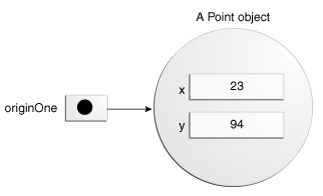
\includegraphics[width=0.6\linewidth]{figs/objects-oneRef.png}
	\end{block}
	\end{columns}
\end{frame}

\begin{frame}[shrink]{Objects}{Creating objects (II)}
%	\vspace{-0.4cm}
	\begin{itemize}
	\item The \texttt{new} operator creates a new object
		\begin{enumerate}
		\item It requires a constructor
		\item It returns a reference
		\end{enumerate}
	\item Valid usages of new
		\begin{enumerate}
		\item \texttt{Point originOne = new Point(23, 94);}
		\item \texttt{int height = new Rectangle().height;}
		\end{enumerate}
	\end{itemize}
	%\footnotesize{
    %\begin{columns}
 	%   \column{.50\textwidth}
	%\vspace{-0.2cm}
	%\begin{block}{Point.java}
%		\vspace{-0.2cm}
%		\lstinputlisting{code/Point.java}[basicstyle=\tiny]
%		\vspace{-0.2cm}
%	\end{block}

 % 	\column{.50\textwidth}
%	\vspace{-0.5cm}
%	\begin{block}{Memory}
%		\tiny{
%		\texttt{Point originOne = new Point(23, 94);}
%		}
%		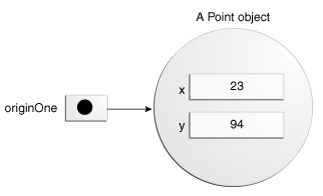
\includegraphics[width=0.7\linewidth]{figs/objects-oneRef.png}
%	\end{block}
%	\end{columns}
%	}
\end{frame}

%\begin{frame}[shrink]{Objects}{Creating objects (V)}
%	\vspace{-0.2cm}
%	\begin{block}{Rectangle.java}
%	\vspace{-0.2cm}
%		\lstinputlisting{code/Rectangle.java}
%	\end{block}
%\end{frame}

%\begin{frame}[shrink]{Objects}{Creating objects (VI)}
%		\centering \texttt{Point rectOne = new Rectangle(originOne, 100, 200);}
%		\bigskip
%		\begin{center}
%		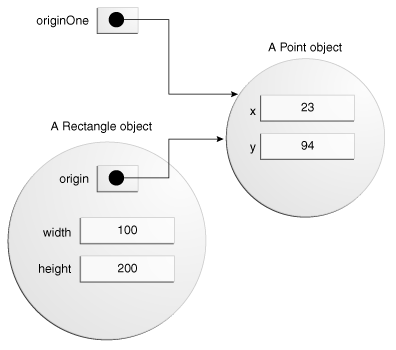
\includegraphics[width=0.5\linewidth]{figs/objects-multipleRefs.png}
%		\end{center}
%\end{frame}

\subsection{Using objects}
\begin{frame}{Objects}{Using objects}
	\begin{itemize}
	\item Fields:
	\begin{itemize}
		\item Within the object: \texttt{width;}
		\item Outside the object: \texttt{object.width;}
	\end{itemize}
	\item Methods
		\begin{itemize}
		\item Within the object: \texttt{getArea();}
		\item Outside the object: \texttt{object.getArea();}
		\end{itemize}
	\item Be careful with private scope!
	\item A good thing about Java: \alert{Garbage collector}
		\begin{itemize}
		\item When an object is no longer referenced, the garbage collector frees its memory automatically
		\item It is invoked by JVM periodically
		\end{itemize}
	\item Delete an object just assigning it \texttt{null}
	\end{itemize}
\end{frame}

\section{More on classes}
\subsection{Returning a value from a method}

\begin{frame}[shrink]{More on classes}{Returning a value from a method}
	\begin{itemize}
	\item A method finishes when first:
	\begin{itemize}
		\item Executes the last statement in the method
		\item Executes a \alert{return} statement
		\item Throws an exception
	\end{itemize}
	\item The return statement indicates the return value
		\begin{itemize}
		\item ... unless the return type is \alert{void}
		\end{itemize}
	\end{itemize}
	\begin{columns}
  	\column{.70\textwidth}
	\vspace{-0.3cm}
	\begin{block}{Example}
		\vspace{-0.2cm}
		\lstinputlisting[language=java, basicstyle=\ttfamily\scriptsize]{code/methods.java}
		\vspace{-0.2cm}
	\end{block}
	\end{columns}

\end{frame}

\subsection{Using the this keyword}

\begin{frame}[shrink]{More on classes}{Using the this keyword}
	The keyword \alert{this} represents the current object

	\begin{columns}
  	\column{.70\textwidth}
	\vspace{-0.2cm}
	\begin{block}{Point.java}
		\vspace{-0.2cm}
		\lstinputlisting[language=java, basicstyle=\ttfamily\scriptsize]{code/pointthis.java}
		\vspace{-0.2cm}
	\end{block}
	\end{columns}
\end{frame}

\subsection{Access control}

\begin{frame}[shrink]{More on classes}{Access control}
	\begin{center}
  	\begin{tabular}{|l|c|c|c|c|}
      	\hline
	 Modifier 	& Class & Package & Subclass& World\\ \hline
	 Public 		& Y 	& Y 	  & Y		& Y	\\ \hline
	 Protected 	& Y 	& Y 	  & Y		& N	\\ \hline
	 No modifier & Y 	& Y 	  & N		& N	\\ \hline
	 Private 	& Y 	& N 	  & N		& N	\\ \hline
	 \end{tabular}
	\end{center}

	\vspace{-0.3cm}
	\begin{block}{Good practices}
		\begin{itemize}
		\item Use the most restrictive access level (\texttt{private} by default)
		\item Avoid \texttt{public} fields except for constants
		\end{itemize}
	\end{block}
\end{frame}

\subsection{The static keyword}

\begin{frame}[shrink]{More on classes}{The static keyword}
	\begin{itemize}
		\item The meaning of \alert{static} depends
		\begin{itemize}
		\item Fields: Field shared by all the objects of that class
			\begin{itemize}
			\item Example: \texttt{public static double PI = 3.14;}
			\item Example: \texttt{System.out}
			\end{itemize}
		\item Methods: They can be invoked without an object
			\begin{itemize}
			\item Example: \texttt{System.out.println()}
			\end{itemize}
		\end{itemize}
		\item Both require the class name:\\\texttt{area = Math.pow(r, 2) * MyClass.PI}
		\item The keyword \alert{final} defines a constant field
		\begin{itemize}
		\item Example: \texttt{public final ruedas = 4;}
		\item Example: \texttt{public static final double PI = 3.14;}
		\end{itemize}

	\end{itemize}
\end{frame}

\section{Inheritance}
\subsection{Definitions}

\begin{frame}[shrink]{Inheritance}{Definitions}
	\begin{itemize}
		\item Objective: Derive your new class from an existing class (reusing its code)
		\begin{itemize}
		\item Subclass, derived class, extended class or child class
		\item Superclass, base class or parent class
		\end{itemize}
		\item Any Java class has a superclass
		\begin{itemize}
		\item The only exception is \texttt{Object}
		\item Any class is derived from \texttt{Object} (\texttt{java.lang.Object})
		\end{itemize}
	\end{itemize}
	
	\begin{center} 
		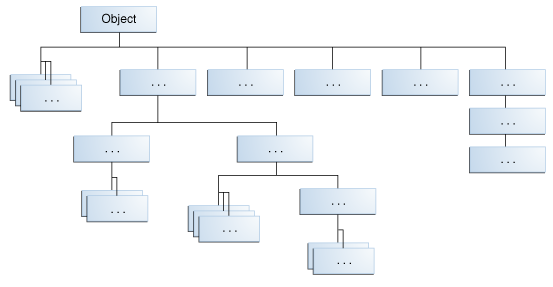
\includegraphics[width=0.5\linewidth]{figs/classes-object.png}
	\end{center}
\end{frame}

\subsection{Inheritance example}
\begin{frame}[shrink]{Inheritance}{Inheritance example (I)}
	\vspace{-0.2cm}
	\begin{block}{Bicycle.java}
		\vspace{-0.2cm}
		\lstinputlisting[language=java, basicstyle=\ttfamily\scriptsize]{code/BicycleBis.java}
		\vspace{-0.2cm}
	\end{block}
\end{frame}

\begin{frame}[shrink]{Inheritance}{Inheritance example (II)}
	\vspace{-0.2cm}
	\begin{block}{MountainBike.java}
		\vspace{-0.2cm}
		\lstinputlisting[language=java, basicstyle=\ttfamily\scriptsize]{code/MountainBike.java}
		\vspace{-0.2cm}
	\end{block}
\end{frame}

\subsection{Overriding and Hiding Methods}
\begin{frame}[shrink]{Inheritance}{Overriding and hiding methods (I)}
	\begin{itemize}
	\item Sometimes we need to adapt the behaviour of an inheritanced method: \alert{Overriding}
	\begin{itemize}
	\item You might want to use \alert{@override} to avoid warnings
	\end{itemize}

	\end{itemize}

	\vspace{-0.2cm}
	\begin{block}{Animal.java}
		\vspace{-0.2cm}
		\lstinputlisting[language=java, basicstyle=\ttfamily\scriptsize]{code/Animal.java}
		\vspace{-0.2cm}
	\end{block}
\end{frame}

\begin{frame}[shrink]{Inheritance}{Overriding and hiding methods (II)}
	\vspace{-0.2cm}
	\begin{block}{Cat.java}
		\vspace{-0.2cm}
		\lstinputlisting[language=java, basicstyle=\ttfamily\scriptsize]{code/Cat.java}
		\vspace{-0.2cm}
	\end{block}
\end{frame}

\subsection{Polymorphism}
\begin{frame}{Inheritance}{Polymorphism (I)}
	\begin{itemize}
	\item \textbf{Polymorphism}: Same method signature, diferent implementations
	\item Define a method in a base class
	\begin{itemize}
	\item Redefine the same method in several subclasses
	\item They can be invoked regardless of the class
	\end{itemize}
	\end{itemize}

	\begin{center} 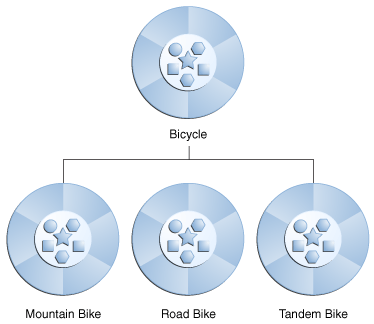
\includegraphics[width=0.4\linewidth]{figs/concepts-bikeHierarchy.png}
	\end{center}
\end{frame}

\begin{frame}{Inheritance}{Polymorphism (II)}
	\begin{itemize}
	\item Example: A superclass (\texttt{Bicycle}) with three subclasses
		\begin{itemize}
		\item \texttt{Bicycle} implements a \texttt{printDescription()} method
		\item Subclasses override \texttt{printDescription()}
		\end{itemize}
	\end{itemize}

	\vspace{-0.2cm}
	\begin{block}{TestBikes.java}
		\vspace{-0.2cm}
		\lstinputlisting[language=java, basicstyle=\ttfamily\scriptsize]{code/TestBikes.java}
		\vspace{-0.2cm}
	\end{block}
\end{frame}

\subsection{Object as superclass}
\begin{frame}{Inheritance}{Object as superclass}
	\begin{itemize}
	\item The class \texttt{Object} is the root of the Java hierarchy
	\item Any Java class inherits a set of methods from \texttt{Object}
	\begin{itemize}
		\item \texttt{protected Object clone() throws CloneNotSupportedException}
		\item \texttt{public boolean equals(Object obj)}
		\item \texttt{protected void finalize() throws Throwable}
		\item \texttt{public final Class getClass()}
		\item \texttt{public int hashCode()}
		\item \texttt{public String toString()}
	\end{itemize}
	\end{itemize}
\end{frame}

\subsection{Abstract methods and classes}
\begin{frame}{Inheritance}{Abstract methods and classes (I)}
	\begin{itemize}
	\item Java supports abstract methods and classes
	\item \textbf{Abstract class}: A class that cannot be instanciated
		\begin{itemize}
		\item Provide a base to develop a class hierarchy
		\item It contains common code
		\end{itemize}
	\item \textbf{Abstract method}: A method without implementation
		\begin{itemize}
		\item It must be overriden by subclasses
		\item It defines a shared behaviour
		\end{itemize}
	\end{itemize}
\end{frame}

\begin{frame}{Inheritance}{Abstract methods and classes (II)}
	\begin{center} 
		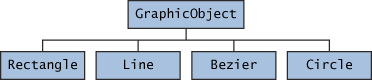
\includegraphics[width=0.5\linewidth]{figs/classes-graphicObject.png}
	\end{center}
	\vspace{-0.2cm}
	\begin{block}{GraphicObject.java}
		\vspace{-0.2cm}
		\lstinputlisting[language=java, basicstyle=\ttfamily\scriptsize]{code/GraphicObject.java}
		\vspace{-0.2cm}
	\end{block}
\end{frame}

\begin{frame}{Inheritance}{Abstract methods and classes (III)}
	\begin{center} 
		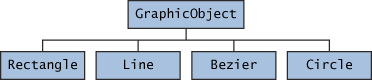
\includegraphics[width=0.5\linewidth]{figs/classes-graphicObject.png}
	\end{center}

	\vspace{-0.2cm}
	\begin{block}{Circle.java}
		\vspace{-0.2cm}
		\lstinputlisting[language=java, basicstyle=\ttfamily\scriptsize]{code/Circle2.java}
		\vspace{-0.2cm}
	\end{block}

	%\vspace{-0.2cm}
	%\begin{block}{Rectangle.java}
	%	\vspace{-0.2cm}
	%	\lstinputlisting{code/Rectangle2.java}
	%	\vspace{-0.2cm}
	%\end{block}

\end{frame}





\end{document}
